\documentclass{article}
\usepackage{tikz}
\usetikzlibrary{shapes.geometric}
\tikzset{triangle/.style={
		regular polygon,
		regular polygon sides=3,
		minimum size=0.5cm,
		draw,
		fill=green}
	}
\begin{document}
	\begin{tabular}{c c c}
		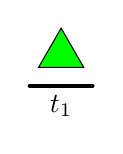
\begin{tikzpicture}[scale=0.4]
			\draw[line cap=round,line width=0.5mm, rounded corners] (0,0) -- (2,0);
			\node [triangle] at (1,1) {} ;
			\node [below] at (1,0) {$t_1$};
		\end{tikzpicture}
	&
		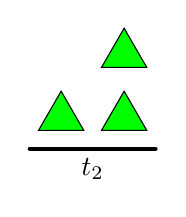
\begin{tikzpicture}[scale=0.4]
			\draw[line cap=round,line width=0.5mm, rounded corners] (0,0) -- (4,0);
			\node [triangle] at (1,1) {} ;
			\node [triangle] at (3,1) {} ;
			\node [triangle] at (3,3) {} ;
			\node [below] at (2,0) {$t_2$};
		\end{tikzpicture}
	&
		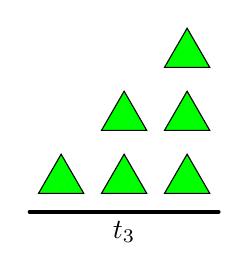
\begin{tikzpicture}[scale=0.4]
			\draw[line cap=round,line width=0.5mm, rounded corners] (0,0) -- (6,0);
			\node [triangle] at (1,1) {} ;
			\node [triangle] at (3,1) {} ;
			\node [triangle] at (3,3) {} ;
			\node [triangle] at (5,1) {} ;
			\node [triangle] at (5,3) {} ;
			\node [triangle] at (5,5) {} ;
			\node [below] at (3,0) {$t_3$};
		\end{tikzpicture}
	\end{tabular}
	
\end{document}